% Phân tích chuyên sâu (2): bộ kiểm tra chiến thuật. \input trong 04-thuc-nghiem.tex.
\section{Bộ kiểm tra chiến thuật}
\label{sec:cs-chien-thuat}
Giải đấu cho biết ai thắng nhưng không cho biết tác tử yếu ở loại tình huống nào. Mục này chấm các tác tử trên một bộ
thế cố định có đáp án kiểm được bằng engine, rồi đổi lần lượt ngân sách và từng tham số.

\subsection{Cách dựng bộ thế}
Nguồn là mọi thế sau khai cuộc của RR8 và E3 trên khai cuộc giữ riêng (88\,849 thế). Danh sách được xáo bằng seed 2026
rồi duyệt; mỗi thế được xếp vào loại đầu tiên nó thoả:
\begin{description}
  \item[C1, thắng ngay.] Bên đi có ô thắng. Đáp án: các ô thắng.
  \item[C2, chặn.] Đối thủ có đúng một ô thắng, bên đi không có. Đáp án: ô đó.
  \item[C3, đòn kép.] Có VCF dài đúng 2 nước tấn công. Đáp án: mọi nước mở đầu một VCF.
  \item[C4, chuỗi tứ.] VCF ngắn nhất dài từ 3 nước. Đáp án như C3.
  \item[C5, phòng thủ.] Bên đi không có đường thắng, nhưng đối thủ sẽ có VCF nếu bên đi bỏ lượt. Đáp án: mọi nước mà
  sau đó đối thủ không còn VCF.
\end{description}
Thế trùng nhau qua đối xứng D4 bị loại, mỗi ván góp tối đa một thế mỗi loại, và mỗi loại lấy đủ 100 thế (đạt sau khi
quét 3\,855 thế). Bảng~\ref{tab:cs-bo-mo-ta} mô tả bộ; Phụ lục~\ref{app:chien-thuat} in toàn bộ.
\begin{table}[H]
  \centering
  \footnotesize
  \caption{Đặc trưng năm loại thế của bộ kiểm tra chiến thuật}
  \label{tab:cs-bo-mo-ta}
  \begin{tabular}{lrrrrrrr}
    \toprule
    Loại & Số thế & Nước thứ & Ứng viên & Đáp án & Max & Ngẫu nhiên (\%) & Độ dài VCF \\
    \midrule
    C1 thắng ngay & 100 & 31,7 & 70,8 & 1,8 & 9 & 2,7 & 1,00 \\
    C2 chặn & 100 & 28,6 & 67,3 & 1,0 & 1 & 1,6 & 0,00 \\
    C3 đòn kép & 100 & 23,4 & 74,5 & 4,3 & 13 & 5,8 & 2,00 \\
    C4 chuỗi tứ & 100 & 26,5 & 73,2 & 3,7 & 12 & 5,0 & 3,82 \\
    C5 phòng thủ & 100 & 16,8 & 62,9 & 3,6 & 16 & 5,8 & 2,13 \\
    \bottomrule
  \end{tabular}
  \par\smallskip\parbox{.95\linewidth}{\footnotesize Các cột 3--5 và 7--8 là trung bình. ``Ngẫu nhiên'' là xác suất trúng khi chọn đều trong tập ứng viên bán kính 2 (ước lượng bằng số đáp án chia số ứng viên). Với C5, độ dài VCF là của đối thủ.}
\end{table}


Ba giới hạn cần giữ khi đọc kết quả. Thứ nhất, đáp án C3, C4 chỉ gồm đường thắng bằng tứ liên tiếp; nước thắng bằng
cách khác bị tính sai, nên tỷ lệ ở hai loại này là cận dưới. Thứ hai, thế lấy từ ván của chính các tác tử được chấm,
nên phân bố thế phản ánh lối chơi của chúng. Thứ ba, mỗi tác tử chạy một seed mỗi thế.

\subsection{Cấu hình giải đấu}
Cấu hình trùng RR8 giữ riêng: L3 độ sâu 4, L4 400 mô phỏng rollout ngẫu nhiên, L7 và L8 200 mô phỏng.
\begin{table}[H]
  \centering
  \small
  \caption{Tỷ lệ chọn đúng (\%) trên bộ chiến thuật, cấu hình giải đấu (chế độ B)}
  \label{tab:cs-ct-goc}
  \begin{tabular}{lrrrrrr}
    \toprule
    Tác tử / cấu hình & C1 & C2 & C3 & C4 & C5 & Tổng \\
    \midrule
    L1 Random & 1 & 1 & 6 & 6 & 8 & 4,4 \\
    L2 Rule & 100 & 100 & 100 & 42 & 89 & 86,2 \\
    L3 AlphaBeta & 100 & 100 & 100 & 83 & 98 & 96,2 \\
    L4 MCTS & 76 & 15 & 24 & 13 & 22 & 30,0 \\
    L5 PolicySL & 80 & 99 & 99 & 90 & 93 & 92,2 \\
    L6 PolicyRL & 90 & 99 & 97 & 84 & 93 & 92,6 \\
    L7 PUCT & 98 & 94 & 100 & 86 & 94 & 94,4 \\
    L8 AlphaZero & 99 & 99 & 100 & 89 & 95 & 96,4 \\
    \bottomrule
  \end{tabular}
\end{table}

L8 ($96{,}4\%$) và L3 ($96{,}2\%$) dẫn đầu, sát nhau. L2 đúng tuyệt đối ở C1--C3 vì đó chính là các luật P1--P3, nhưng chỉ
đạt $42\%$ ở C4. L5 và L6, không tìm kiếm, vẫn đạt khoảng $92\%$, cho thấy mạng đã học phần lớn phản xạ chiến thuật
một đến hai nước. Điểm yếu riêng của L5 là C1 ($80\%$), dấu vết của lỗi nhãn ở Mục~\ref{sec:cs-du-lieu}.

\begin{table}[H]
  \centering
  \small
  \caption{So sánh ghép cặp trên cùng 500 thế (kiểm định McNemar chính xác)}
  \label{tab:cs-ct-mcnemar}
  \begin{tabular}{lrrrrr}
    \toprule
    Cặp A / B & Cả hai đúng & Chỉ A & Chỉ B & Cả hai sai & $p$ \\
    \midrule
    L5 / L6 & 446 & 15 & 17 & 22 & 0,860 \\
    L3 / L7 & 460 & 21 & 12 & 7 & 0,163 \\
    L7 / L8 & 464 & 8 & 18 & 10 & 0,076 \\
    L5 / L7 & 448 & 13 & 24 & 15 & 0,099 \\
    L2 / L5 & 401 & 30 & 60 & 9 & 0,002 \\
    \bottomrule
  \end{tabular}
\end{table}

Kiểm định McNemar chỉ cho thấy L5 hơn L2 một cách rõ ($p\approx0{,}002$). Các cặp còn lại, kể cả L7--L8, chưa phân biệt
được trên 500 thế, dù khi đấu chúng khác nhau rõ: bộ thế đo chiến thuật ngắn, trong khi chênh lệch sức chơi giữa các
cấp mạnh nằm nhiều ở nước yên tĩnh.
\begin{table}[H]
  \centering
  \small
  \caption{Số thế theo số tác tử (trong tám) chọn đúng}
  \label{tab:cs-ct-dokho}
  \begin{tabular}{crrrrrr}
    \toprule
    Số tác tử đúng & C1 & C2 & C3 & C4 & C5 & Tổng \\
    \midrule
    0 & 0 & 0 & 0 & 1 & 0 & 1 \\
    1 & 0 & 0 & 0 & 2 & 3 & 5 \\
    2 & 0 & 0 & 0 & 5 & 2 & 7 \\
    3 & 1 & 1 & 0 & 3 & 0 & 5 \\
    4 & 2 & 0 & 0 & 16 & 2 & 20 \\
    5 & 6 & 6 & 3 & 37 & 4 & 56 \\
    6 & 35 & 77 & 70 & 30 & 68 & 280 \\
    7 & 55 & 16 & 25 & 5 & 19 & 120 \\
    8 & 1 & 0 & 2 & 1 & 2 & 6 \\
    \bottomrule
  \end{tabular}
\end{table}

Phần lớn thế được 6 hoặc 7 trong 8 tác tử giải đúng (thường chỉ L1 và L4 sai). Các thế khó, được không quá bốn tác tử
giải, tập trung ở C4. Một thế không tác tử nào giải được.

\subsection{Cấp 3 theo độ sâu}
\begin{table}[H]
  \centering
  \small
  \caption{L3: tỷ lệ chọn đúng (\%) theo độ sâu tìm kiếm}
  \label{tab:cs-ct-l3}
  \begin{tabular}{lrrrrrr}
    \toprule
    Tác tử / cấu hình & C1 & C2 & C3 & C4 & C5 & Tổng \\
    \midrule
    độ sâu, 1 & 100 & 54 & 100 & 96 & 81 & 86,2 \\
    độ sâu, 2 & 100 & 100 & 98 & 86 & 100 & 96,8 \\
    độ sâu, 3 & 100 & 100 & 100 & 93 & 87 & 96,0 \\
    độ sâu, 4 & 100 & 100 & 100 & 83 & 98 & 96,2 \\
    độ sâu, 5 & 100 & 100 & 100 & 89 & 97 & 97,2 \\
    độ sâu, 6 & 100 & 100 & 100 & 90 & 98 & 97,6 \\
    \bottomrule
  \end{tabular}
\end{table}

\begin{figure}[H]
  \centering
  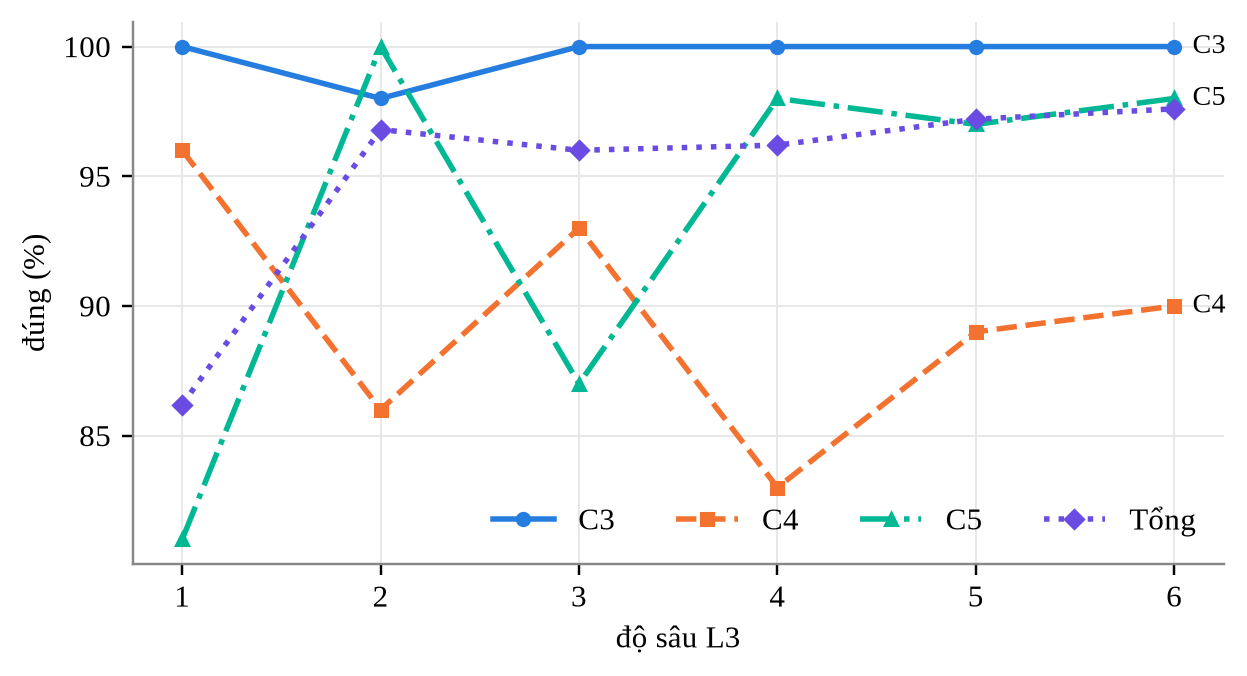
\includegraphics[width=0.82\linewidth]{chuyen-sau/hinh/ct-l3-dosau.png}
  \caption{Tỷ lệ đúng của L3 theo độ sâu ở ba loại khó.}
  \label{fig:cs-ct-l3}
\end{figure}
Độ sâu 1 chỉ đạt $54\%$ ở C2: gốc không áp dụng nước bắt buộc, và lá ở độ sâu 1 không thấy đối thủ thắng ngay sau đó,
đúng như phân tích mã ở Mục~\ref{sec:cs-cai-dat}. Từ độ sâu 2, C2 đạt $100\%$. Ở C4 và C5, tỷ lệ \emph{không đơn điệu}
theo độ sâu: C4 đạt $93\%$ ở độ sâu 3 nhưng $83\%$ ở độ sâu 4; C5 đạt $100\%$ ở độ sâu 2 nhưng $87\%$ ở độ sâu 3. Hai
nguyên nhân có thể: hàm lượng giá ở lá lệch theo tính chẵn lẻ của độ sâu (bên vừa đi có thêm một quân), và ở C4 một
phần nước ``sai'' có thể vẫn thắng bằng đường ngoài VCF. Đề tài chưa tách hai nguyên nhân.

\subsection{MCTS theo ngân sách và kiểu rollout}
\begin{table}[H]
  \centering
  \footnotesize
  \caption{MCTS: tỷ lệ chọn đúng (\%) theo kiểu rollout và số mô phỏng}
  \label{tab:cs-ct-l4}
  \begin{tabular}{lrrrrrr}
    \toprule
    Tác tử / cấu hình & C1 & C2 & C3 & C4 & C5 & Tổng \\
    \midrule
    ngẫu nhiên, 100 & 7 & 5 & 8 & 9 & 17 & 9,2 \\
    ngẫu nhiên, 400 & 76 & 15 & 24 & 13 & 22 & 30,0 \\
    ngẫu nhiên, 800 & 95 & 20 & 42 & 27 & 35 & 43,8 \\
    ngẫu nhiên, 1600 & 100 & 40 & 76 & 42 & 41 & 59,8 \\
    ngẫu nhiên, 6400 & 100 & 73 & 98 & 76 & 65 & 82,4 \\
    \midrule
    light, 100 & 23 & 19 & 21 & 24 & 18 & 21,0 \\
    light, 400 & 23 & 3 & 84 & 76 & 65 & 50,2 \\
    light, 800 & 24 & 4 & 96 & 83 & 76 & 56,6 \\
    light, 1600 & 24 & 4 & 100 & 88 & 81 & 59,4 \\
    light, 6400 & 60 & 74 & 93 & 76 & 92 & 79,0 \\
    \midrule
    light + gốc, 100 & 100 & 100 & 100 & 11 & 80 & 78,2 \\
    light + gốc, 800 & 100 & 100 & 100 & 39 & 89 & 85,6 \\
    light + gốc, 6400 & 100 & 100 & 100 & 34 & 90 & 84,8 \\
    \bottomrule
  \end{tabular}
\end{table}

\begin{figure}[H]
  \centering
  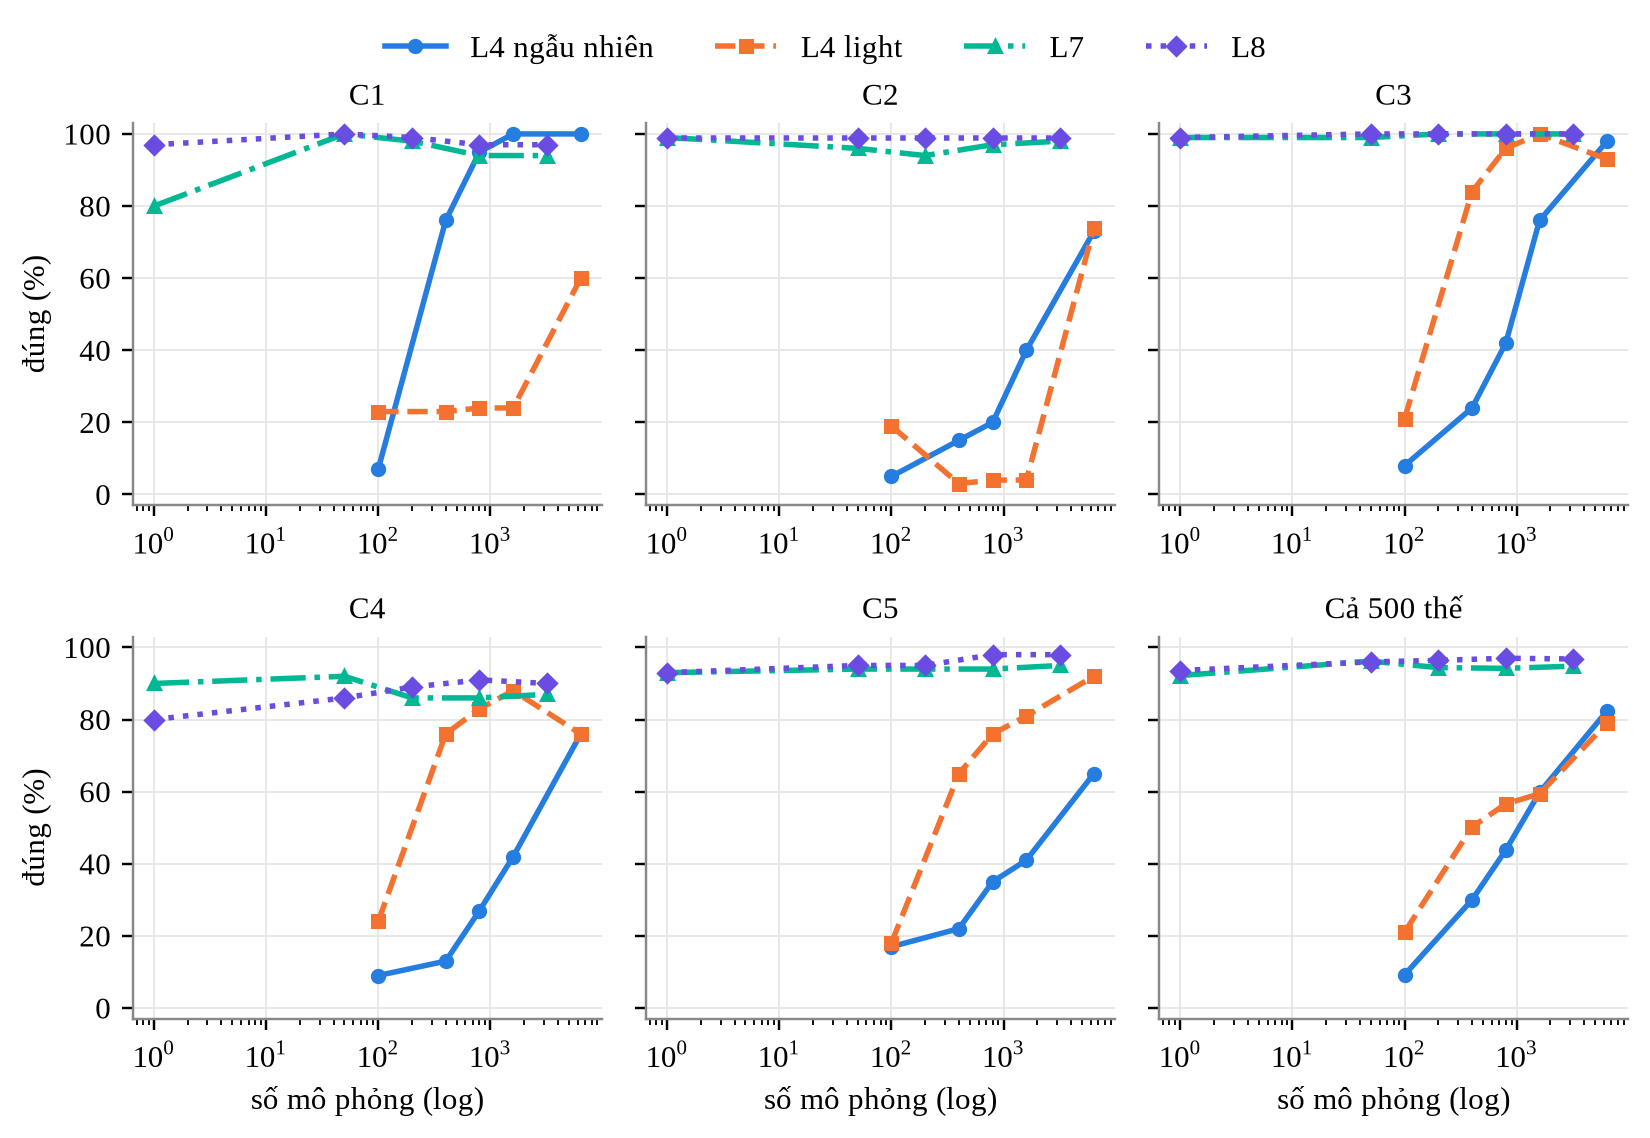
\includegraphics[width=\linewidth]{chuyen-sau/hinh/ct-scale.png}
  \caption{Tỷ lệ đúng theo số mô phỏng (thang log) của MCTS và PUCT trên từng loại thế.}
  \label{fig:cs-ct-scale}
\end{figure}
Rollout ngẫu nhiên cải thiện đều theo ngân sách, từ $9\%$ ở 100 mô phỏng lên $82\%$ ở 6\,400: MCTS hội tụ nhưng chậm,
đúng với cận mẫu ở định lý~\ref{dl:cs-hoeffding}. Rollout \texttt{light} cho hai kết quả trái trực giác.

\paragraph{C1 quanh $23\%$.} Rollout \texttt{light} thắng ngay khi có thể, nên nếu bên đi bỏ qua ô thắng mà vẫn còn hai ô
thắng, mô phỏng sau đó vẫn thắng: nhiều nước yên tĩnh có giá trị $+1$ như nước thắng ngay. Tìm kiếm khi đó chọn một
trong số chúng. Nước được chọn thường vẫn thắng, chỉ chậm hơn; đáp án của C1 không tính nó.

\paragraph{C2 chỉ $3$--$4\%$ ở 400--1\,600 mô phỏng.} Đây gần mức chọn ngẫu nhiên, trong khi rollout ngẫu nhiên đạt
15--40\%. Bảng~\ref{tab:cs-ct-rollout} cho thấy cơ chế.
\begin{table}[H]
  \centering
  \small
  \caption{MCTS rollout light ở 100 thế phải chặn: cây thấy gì khi chọn sai}
  \label{tab:cs-ct-rollout}
  \begin{tabular}{lrr}
    \toprule
    Đại lượng & 400 mô phỏng & 1.600 mô phỏng \\
    \midrule
    Chọn đúng nước chặn & 4/100 & 4/100 \\
    Điểm $Q$ của nước sai được chọn (TB) & 0,84 & 0,44 \\
    Lượt thăm nút đó (TB) & 33,5 & 91,2 \\
    Đáp trả đã mở rộng / tổng (TB) & 32,5 / 70,0 & 69,6 / 71,8 \\
    Đã mở rộng nước thắng của đối thủ & 26/96 & 93/96 \\
    \bottomrule
  \end{tabular}
  \par\smallskip\parbox{.95\linewidth}{\footnotesize Rollout light chạy trực tiếp (200 lần mỗi nước): sau nước chặn trung bình 0,07, sau một nước không chặn trung bình -1,00.}
\end{table}

Chạy rollout trực tiếp, sau một nước không chặn đối thủ thắng ngay ở \emph{mọi} lần (giá trị $-1$). Nhưng trong cây,
mỗi lượt chỉ mở rộng một đáp trả chọn ngẫu nhiên, và đáp trả đó đi trong cây chứ không theo chính sách
\texttt{light}. Khi đối thủ đi một nước khác ô thắng, rollout \texttt{light} của bên ta lập tức \emph{chặn hộ} ô đó; thế
được đánh giá rất tốt. Ở 400 mô phỏng, nút của nước sai được thăm trung bình khoảng 34 lần trong khi có khoảng 70 đáp
trả, nên nước thắng của đối thủ chỉ được mở rộng ở 26 trên 96 trường hợp, và điểm trung bình của nước sai là $+0{,}84$.
Ở 1\,600 mô phỏng, nước thắng đã được mở rộng ở 93/96 trường hợp, nhưng một mẫu $-1$ bị pha loãng giữa hàng chục đáp
trả khác nên điểm vẫn $+0{,}44$. Chỉ khi ngân sách đủ để UCT ở nút đối thủ dồn lượt vào nước thắng (6\,400), tỷ lệ chặn
mới lên $74\%$.

Cơ chế này giải thích quan sát ở A4 và Bảng~\ref{tab:loi-mcts}: với rollout \texttt{light}, tỷ lệ ván thua do bỏ sót chặn
năm \emph{tăng}. Rollout thông minh hơn không giúp, thậm chí hại, nếu nút mở rộng trong cây không dùng cùng tri thức.
Cách sửa chuẩn là ưu tiên mở rộng các đáp trả chiến thuật (thắng ngay trước) hoặc dùng tiên nghiệm như PUCT.

\paragraph{Chiến thuật ở gốc.} Bật \texttt{root\_tactics} đưa C1--C3 lên $100\%$ vì chúng được xử lý bằng luật. Nhưng C4
tụt xuống $11$--$39\%$: khi đối thủ có thể tạo đòn kép, gốc bị giới hạn vào các ô phòng thủ đó, kể cả khi bên đi đang có
chuỗi tứ thắng ép, mà tứ buộc đối thủ phải đáp trước. Đây cùng loại xung đột thứ tự luật với L2 (xem dưới).

\subsection{PUCT theo số mô phỏng}
\begin{table}[H]
  \centering
  \small
  \caption{PUCT: tỷ lệ chọn đúng (\%) theo số mô phỏng}
  \label{tab:cs-ct-puct}
  \begin{tabular}{lrrrrrr}
    \toprule
    Tác tử / cấu hình & C1 & C2 & C3 & C4 & C5 & Tổng \\
    \midrule
    L7, sims, 1 & 80 & 99 & 99 & 90 & 93 & 92,2 \\
    L7, sims, 50 & 100 & 96 & 99 & 92 & 94 & 96,2 \\
    L7, sims, 200 & 98 & 94 & 100 & 86 & 94 & 94,4 \\
    L7, sims, 800 & 94 & 97 & 100 & 86 & 94 & 94,2 \\
    L7, sims, 3200 & 94 & 98 & 100 & 87 & 95 & 94,8 \\
    \midrule
    L8, sims, 1 & 97 & 99 & 99 & 80 & 93 & 93,6 \\
    L8, sims, 50 & 100 & 99 & 100 & 86 & 95 & 96,0 \\
    L8, sims, 200 & 99 & 99 & 100 & 89 & 95 & 96,4 \\
    L8, sims, 800 & 97 & 99 & 100 & 91 & 98 & 97,0 \\
    L8, sims, 3200 & 97 & 99 & 100 & 90 & 98 & 96,8 \\
    \bottomrule
  \end{tabular}
\end{table}

Một mô phỏng tương đương đi theo tiên nghiệm, và L7 ở mức đó đạt đúng $92{,}2\%$ như L5: một phép kiểm tra chéo cho cài
đặt. Chỉ 50 mô phỏng đã nâng L7 lên $96{,}2\%$. Tăng tiếp không cải thiện, L7 thậm chí giảm nhẹ ($94{,}2\%$ ở 800), chủ
yếu ở C1: khi nhiều nước cùng dẫn tới thắng, value đều gần $+1$ và lượt thăm bị chia cho đường thắng chậm. L8 tăng đến
$97{,}0\%$ ở 800 rồi đi ngang. Với chiến thuật ngắn, mạng đã làm phần lớn việc và tìm kiếm chỉ sửa vài phần trăm.

\subsection{Độ nhạy theo tham số}
\begin{table}[H]
  \centering
  \small
  \caption{Ảnh hưởng của $c_{puct}$ (200 mô phỏng), tỷ lệ đúng (\%)}
  \label{tab:cs-ct-cpuct}
  \begin{tabular}{lrrrrrr}
    \toprule
    Tác tử / cấu hình & C1 & C2 & C3 & C4 & C5 & Tổng \\
    \midrule
    L7, c\_puct=0.5 & 100 & 94 & 100 & 85 & 95 & 94,8 \\
    L7, c\_puct=1.0 & 99 & 95 & 100 & 86 & 95 & 95,0 \\
    L7, c\_puct=1.5 & 98 & 94 & 100 & 86 & 94 & 94,4 \\
    L7, c\_puct=3.0 & 97 & 96 & 100 & 90 & 94 & 95,4 \\
    L7, c\_puct=5.0 & 93 & 97 & 100 & 93 & 94 & 95,4 \\
    L8, c\_puct=0.5 & 100 & 99 & 100 & 90 & 97 & 97,2 \\
    L8, c\_puct=1.0 & 100 & 99 & 100 & 89 & 96 & 96,8 \\
    L8, c\_puct=1.5 & 99 & 99 & 100 & 89 & 95 & 96,4 \\
    L8, c\_puct=3.0 & 98 & 99 & 100 & 89 & 94 & 96,0 \\
    L8, c\_puct=5.0 & 97 & 99 & 100 & 89 & 95 & 96,0 \\
    \bottomrule
  \end{tabular}
\end{table}

\begin{table}[H]
  \centering
  \small
  \caption{Ảnh hưởng của số lá gom mỗi lô (200 mô phỏng), tỷ lệ đúng (\%)}
  \label{tab:cs-ct-batch}
  \begin{tabular}{lrrrrrr}
    \toprule
    Tác tử / cấu hình & C1 & C2 & C3 & C4 & C5 & Tổng \\
    \midrule
    L7, batch=1 & 93 & 94 & 100 & 86 & 93 & 93,2 \\
    L7, batch=4 & 97 & 94 & 100 & 89 & 94 & 94,8 \\
    L7, batch=8 & 98 & 94 & 100 & 86 & 94 & 94,4 \\
    L7, batch=16 & 100 & 94 & 100 & 91 & 95 & 96,0 \\
    L7, batch=32 & 100 & 95 & 100 & 93 & 95 & 96,6 \\
    L8, batch=1 & 97 & 99 & 100 & 88 & 94 & 95,6 \\
    L8, batch=4 & 98 & 99 & 100 & 89 & 94 & 96,0 \\
    L8, batch=8 & 99 & 99 & 100 & 89 & 95 & 96,4 \\
    L8, batch=16 & 100 & 99 & 100 & 89 & 96 & 96,8 \\
    L8, batch=32 & 100 & 99 & 100 & 86 & 96 & 96,2 \\
    \bottomrule
  \end{tabular}
\end{table}

\begin{table}[H]
  \centering
  \small
  \caption{L7: trộn giá trị mạng với rollout, tỷ lệ đúng (\%)}
  \label{tab:cs-ct-mix}
  \begin{tabular}{lrrrrrr}
    \toprule
    Tác tử / cấu hình & C1 & C2 & C3 & C4 & C5 & Tổng \\
    \midrule
    L7, mix=0.0 & 98 & 94 & 100 & 86 & 94 & 94,4 \\
    L7, mix=0.5 & 98 & 95 & 100 & 92 & 94 & 95,8 \\
    L7, mix=1.0 & 98 & 99 & 100 & 95 & 97 & 97,8 \\
    \bottomrule
  \end{tabular}
\end{table}

\begin{table}[H]
  \centering
  \small
  \caption{L4 rollout light, 400 mô phỏng: ảnh hưởng của $c_{uct}$}
  \label{tab:cs-ct-cuct}
  \begin{tabular}{lrrrrrr}
    \toprule
    Tác tử / cấu hình & C1 & C2 & C3 & C4 & C5 & Tổng \\
    \midrule
    L4, c\_uct=0.25 & 28 & 62 & 95 & 69 & 54 & 61,6 \\
    L4, c\_uct=0.7 & 28 & 10 & 91 & 78 & 61 & 53,6 \\
    L4, c\_uct=1.4 & 23 & 3 & 84 & 76 & 65 & 50,2 \\
    L4, c\_uct=2.8 & 23 & 8 & 71 & 76 & 60 & 47,6 \\
    \bottomrule
  \end{tabular}
\end{table}

Các khác biệt cỡ 1--2 điểm phần trăm tương ứng 5--10 thế và không đủ để xếp hạng. Những xu hướng đủ lớn để ghi nhận:
\begin{itemize}
  \item $c_{puct}$ trong khoảng $0{,}5$--$5$ ảnh hưởng ít tới tổng; $c$ lớn giảm nhẹ C1 và tăng C4 ở L7, đúng hướng đánh
  đổi khai thác--thăm dò.
  \item Gom lá lớn không làm giảm chất lượng chiến thuật trên bộ này; với L7, 32 lá ($96{,}6\%$) còn cao hơn 1 lá
  ($93{,}2\%$), vì virtual loss buộc tìm kiếm lan rộng hơn khi tiên nghiệm tập trung.
  \item Trộn giá trị mạng với rollout \texttt{light} giúp L7 (từ $94{,}4\%$ lên $97{,}8\%$ khi lá chỉ dùng rollout): ở thế
  chiến thuật, rollout biết thắng và chặn cho tín hiệu lá tốt hơn value head của SL v3.
  \item Với MCTS \texttt{light} ở 400 mô phỏng, $c_{uct}=0{,}25$ ($61{,}6\%$) tốt hơn mức mặc định $1{,}4$ ($50{,}2\%$): khai
  thác nhiều hơn giúp dồn lượt vào đáp trả thắng ở nút đối thủ.
\end{itemize}

\subsection{Bỏ từng luật và đổi tham số Alpha-Beta}
\begin{table}[H]
  \centering
  \small
  \caption{L2: tỷ lệ đúng (\%) khi tắt lần lượt từng luật}
  \label{tab:cs-ct-l2}
  \begin{tabular}{lrrrrrr}
    \toprule
    Tác tử / cấu hình & C1 & C2 & C3 & C4 & C5 & Tổng \\
    \midrule
    L2, -P1 & 2 & 100 & 100 & 42 & 89 & 66,6 \\
    L2, -P2 & 100 & 12 & 100 & 42 & 89 & 68,6 \\
    L2, -P3 & 100 & 100 & 65 & 42 & 89 & 79,2 \\
    L2, -P4 & 100 & 100 & 100 & 96 & 81 & 95,4 \\
    L2, -P5 & 100 & 100 & 100 & 42 & 89 & 86,2 \\
    L2, -P6 & 100 & 100 & 100 & 42 & 89 & 86,2 \\
    \bottomrule
  \end{tabular}
\end{table}

\begin{table}[H]
  \centering
  \small
  \caption{L3 độ sâu 4: tỷ lệ đúng (\%) khi đổi từng tham số}
  \label{tab:cs-ct-l3bien}
  \begin{tabular}{lrrrrrr}
    \toprule
    Tác tử / cấu hình & C1 & C2 & C3 & C4 & C5 & Tổng \\
    \midrule
    L3, no\_forced & 100 & 100 & 100 & 86 & 98 & 96,8 \\
    L3, no\_defense & 100 & 100 & 100 & 87 & 95 & 96,4 \\
    L3, radius=1 & 100 & 100 & 100 & 80 & 97 & 95,4 \\
    \bottomrule
  \end{tabular}
\end{table}

Tắt P1, P2, P3 làm sụp đúng loại tương ứng (C1 còn $2\%$, C2 $12\%$, C3 $65\%$). Tắt P4 làm C4 \emph{tăng} từ $42\%$ lên
$96\%$ và C5 giảm từ $89\%$ xuống $81\%$. P4 đứng trước P5: hễ đối thủ có khả năng tạo đòn kép, L2 đi phòng thủ, kể cả
khi có thể tạo tứ và giữ quyền chủ động. Đưa điều kiện ``đang có chuỗi tứ'' lên trước P4 là cải tiến rõ ràng, chưa thử
khi đấu. Tắt P6 không đổi gì theo cấu trúc mã: P7 chọn trong cùng tập nước điểm cao nhất. Tắt P5 chỉ đổi nước ở 1/500 thế: khi P5
đáng lẽ áp dụng, P4 thường đã quyết định trước, hoặc P6 chọn cùng nước.

Với Alpha-Beta độ sâu 4, tắt nước bắt buộc, bỏ thành phần phòng thủ trong lượng giá hay thu bán kính ứng viên còn 1 đều
đổi tổng không quá $1$ điểm phần trăm. Bán kính 1 giảm C4 từ $83\%$ xuống $80\%$, vì có đường tứ bắt đầu ở ô cách quân
gần nhất hai ô.
